\chapter{实验结果和分析}
\section{静态实验}
\subsection{断裂模式分析}
\begin{figure}
\centering   
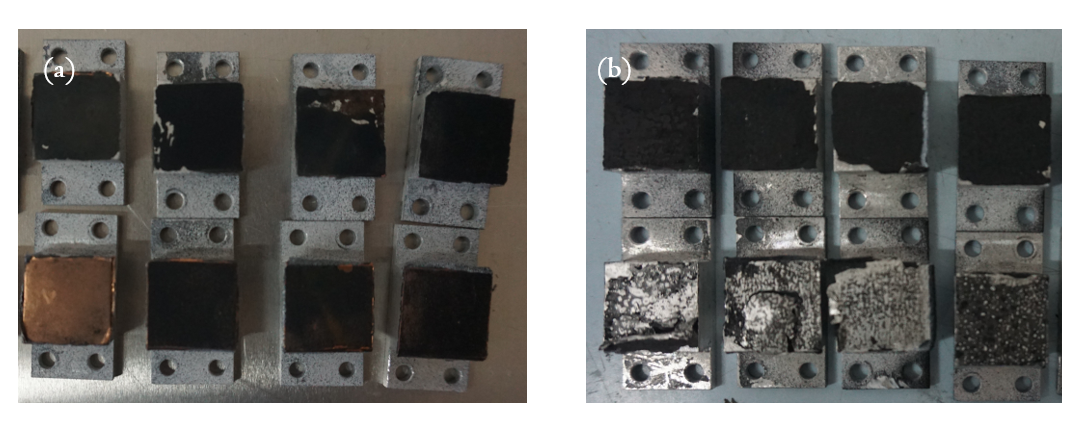
\includegraphics[width=\textwidth]{failure_ac.png}
\caption{正负极拉伸实验样品断裂图} 
\label{fig:ac}
\end{figure}
\begin{figure}
\centering   
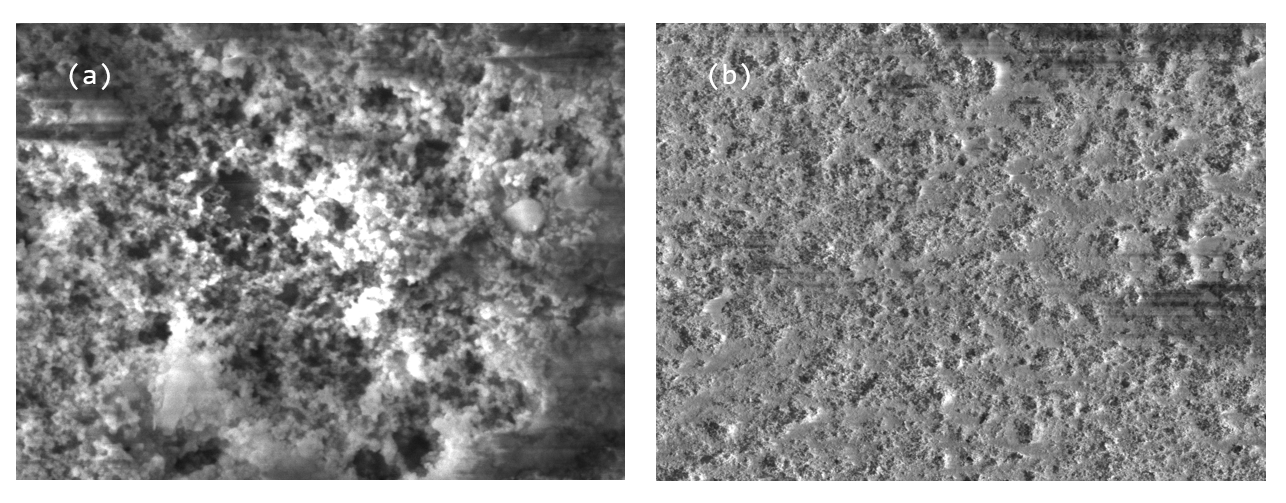
\includegraphics[width=\textwidth]{SEM.png}
\caption{样品断裂面的电镜照片:(a)活性物质侧 (b)金属箔侧} 
\label{fig:sem}
\end{figure}
按照第3章中所介绍的实验设计我们分别进行了电池正极和负极的从$0^{\circ}$到$90^{\circ}$的静态加载测试,实验中得到的正极和负极样品的断面如图\ref{fig:ac}所示。同时,也对实验后的断面进行了扫描电镜的检查,其结果如图\ref{fig:sem}所示。
可以看出,对于所有的样品都得到了所设定的在凝胶侧的集流体和活性层的脱层失效的断裂模态。 但是比较不同角度的加载测试,其测试结果却呈现出复杂的混合拉伸-剪切失效模态。 从$0^{\circ}$到$90^{\circ}$,失效模态发生了显著的变化。 对于$90^{\circ}$拉伸即单向拉伸测试,粘接失效是主要的失效模态,而在试验中可以观测到几乎所有的活性颗粒都会从集流体上脱落,而对于$0^{\circ}$拉伸测试即纯剪测试而言,活性层会有相当部分附着在集流体上只有一小部分集流体清晰可见。 可以看出前文所提到的失效模式中的Cohesion(即活性层内部的断裂失效)和Adhesion(活性层和集流体之间的脱层失效)两种失效模式在其中均发挥着作用。而考虑到之前所提到的活性层中粘结剂的法向分布\cite{M2017Investigation},在所有的加载角度,Adhesion失效模态应该都是主导的失效模式。如图\ref{fig:mech}所示,靠近底层的颗粒的胶层的厚度要比其他层要薄一些,虽然这样会得到最内层最为薄弱的结论,但是其实对于最内层而言,颗粒和集流体金属箔之前的接触面积可能会相对较大,从而对于剪切加载而言\ref{fig:mech}(b),颗粒和活性层之间的剪切强度可能对比垂直方向上颗粒之间的粘接强度要高,从而会造成在剪切实验中,断裂面的集流体一侧上依然会附着有不少的活性物质颗粒。 而随着加载角度的变化,剪切的成分增加,不同深度处的活性层颗粒之前可能会发生的相对滑移和挤压会使得剪切强度增加。 同时,需要指出的是,对于活性层-集流体粘接的界面,其剪切失效强度依然只由粘结剂和粘结剂对集流体和活性颗粒之间的粘接情况相关。
\begin{figure}
\centering   
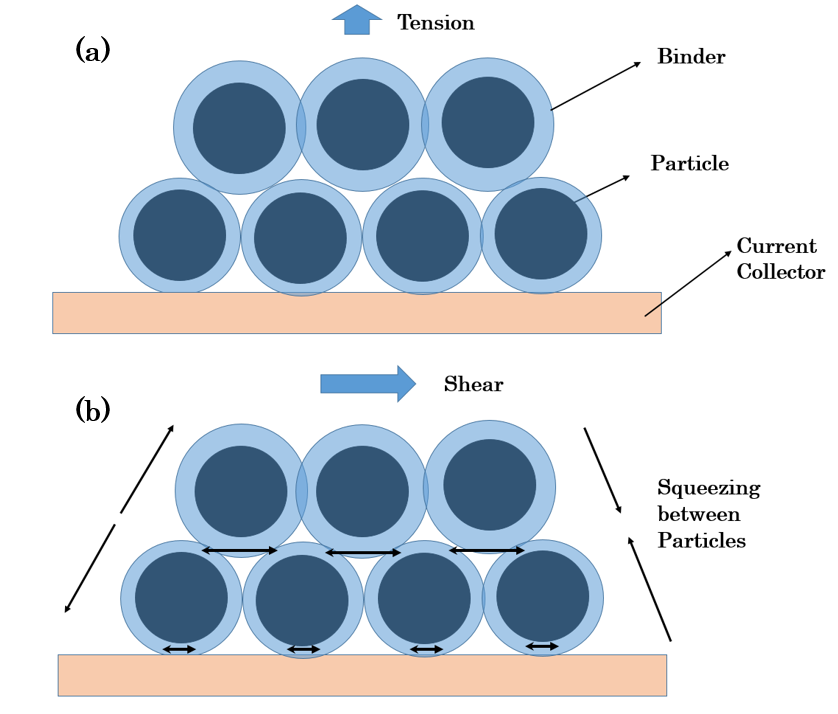
\includegraphics[width=\textwidth]{failure_me.png}
\caption{断裂失效的示意图:(a)拉伸 (b)剪切} 
\label{fig:mech}
\end{figure}
\subsection{不同应力状态下的粘接强度}
所有的实验样品其截面均为$20 \times 20(mm)$,假设应力在截面上均匀分布,则有效断裂强度可以用下式求得:
\begin{equation}
\sigma_{\mu} = F_f/A
\end{equation}
其中,$F_f$是力学加载过程中的峰值力,而$A$为断裂面的面积。电池正极和负极的测试结果分别如图\ref{fig:strength}(a)(b)所示。可以看出,正极和负极的结果呈现出不同的规律:
\begin{itemize}
	\item 对正极而言,断裂强度分布在1.0MPa到2.4MPa之间,从$0^{\circ}$到$60^{\circ}$,断裂强度整体呈现下降趋势,但在$45^{\circ}$处呈现出反常并取得其最大值,而在$75^{\circ}$处也出现了一个极值,可以看出在混合拉伸-剪切的加载下,有着相对较大的剪切分量加载下其粘接强度会有所提升
	\item 对负极而言,断裂强度分布在0.9MPa到2MPa之间,而主要集中分布在1.25MPa上下,只在$15^{\circ}$和$75^{\circ}$处有所反常分别出现了最大值和最小值,这可能是由于负极活性层相比正极而言涂布较薄,失效模态相对集中。
\end{itemize}
总之,电极的粘接强度的混合拉伸-剪切失效呈现出复杂的变化规律,而总体而言正极活性层的粘接强度要显著高于负极的粘接强度,这也和之前的对电池的挤压等测试的结果相一致\cite{Luo2017Mechanical}。
\begin{figure}
\centering   
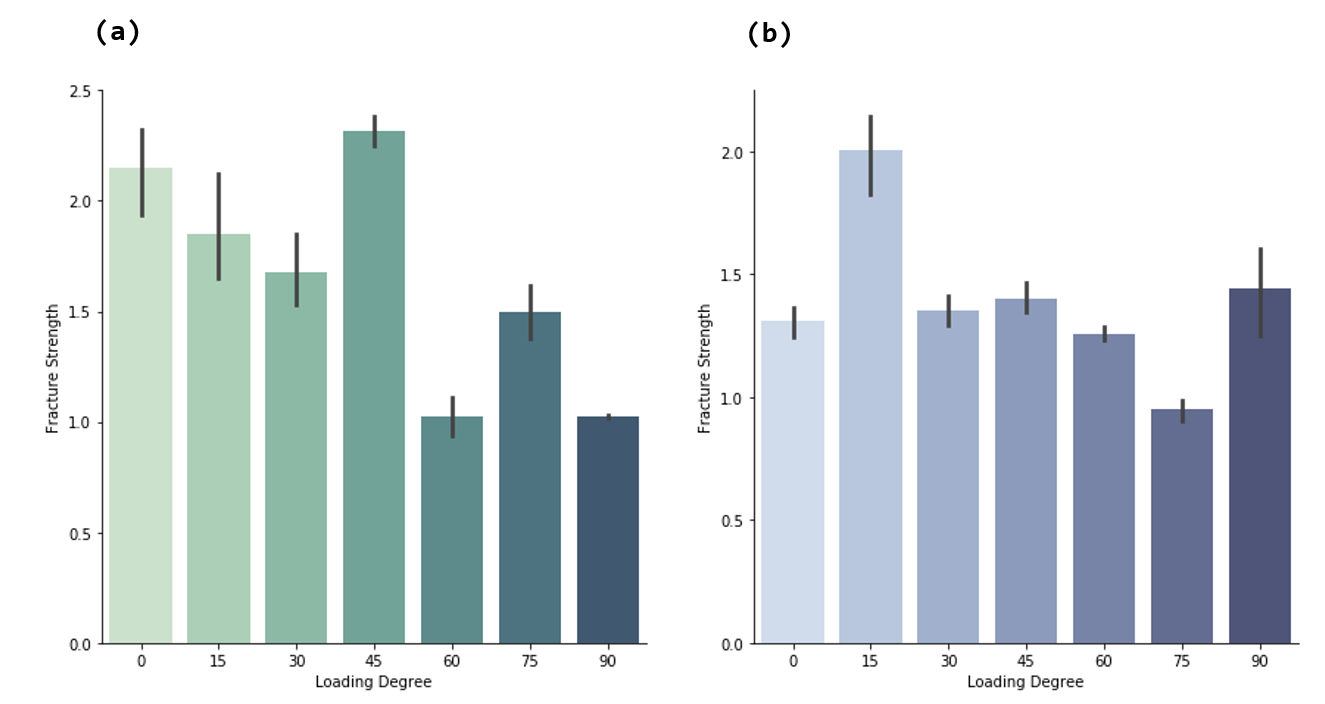
\includegraphics[width=\textwidth]{Strength.png}
\caption{不同角度的粘接强度测试结果:(a)正极 (b)负极} 
\label{fig:strength}
\end{figure}
\indent 对于这一实验,整体的断裂强度可以被分解为拉伸和剪切两个独立分量:
\begin{equation}
\sigma_n =\sigma_{\mu}sin\theta
\end{equation}
\begin{equation}
\sigma_s =\sigma_{\mu}cos\theta
\end{equation}
\begin{figure}
\centering   
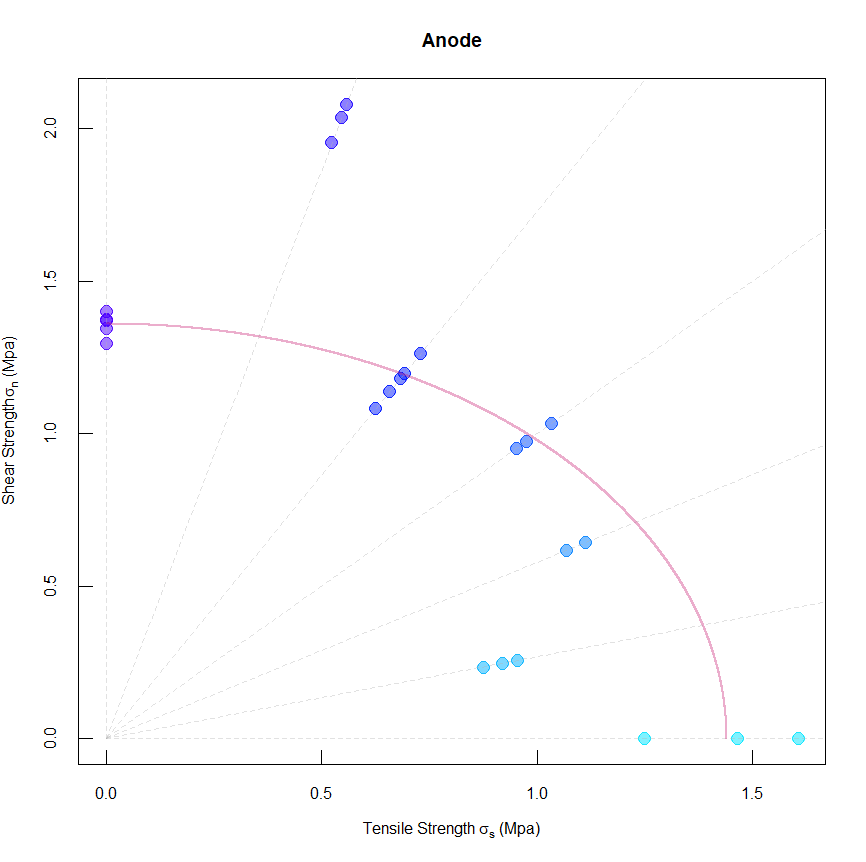
\includegraphics[width=\textwidth]{circle_a.png}
\caption{不同测试的拉伸和剪切分量:正极} 
\label{fig:circle_a}
\end{figure}
\begin{figure}
\centering   
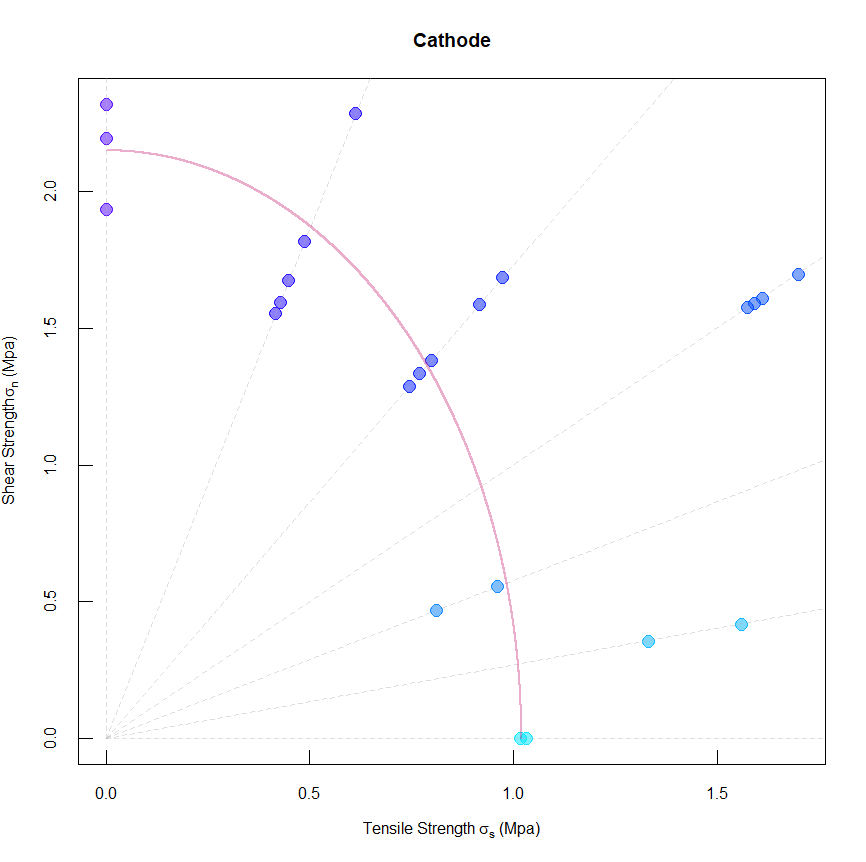
\includegraphics[width=\textwidth]{circle_c.png}
\caption{不同测试的拉伸和剪切分量:负极} 
\label{fig:circle_c}
\end{figure}
其中,$\theta$是加载角度,从$90^{\circ}$到$0^{\circ}$分别从单向拉伸变化到纯剪切加载,而$\sigma_n$和$\sigma_s$分别是拉伸和剪切分量。 可以在$\sigma_n - \sigma_s$平面分别画出结果\ref{fig:circle_a}和\ref{fig:circle_c},并可以采用之前所分析的内聚力模型(Cohesive zone model)来表征粘接失效行为:
\begin{equation}
\left(\frac{\sigma_n}{NFLS} \right)^2 + \left(\frac{\sigma_s}{SFLS} \right)^2 = 1
\end{equation}
两个椭圆线的拟合参数NFLS和SFLS分别为拉伸和剪切的失效应力。 在图\ref{fig:circle_a}\ref{fig:circle_c}中,对正极和负极分别进行拟合绘制出虚线所示的失效线。可以看出对于正极(NFLS = 1.42MPa, SFLS = 1.40MPa)而言,失效线低估了整体的失效行为,而对负极(NFLS = 1.36MPa, SFLS = 1.44MPa)则是相对高估(除去其中$15^{\circ}$的情形)。

\section{动态实验}
除了静态实验之外,对正极和负极还进行了$0.1m/s$和$1m/s$分为$90^{\circ}$,$60^{\circ}$和$30^{\circ}$的加载测试,不同速度下的测试结果如图\ref{fig:a}和\ref{fig:c}所示(动态测试时较高速度下正极铝箔出现明显断裂故没有采用正极的$1m/s$的实验数据)。可以看出,在应变率增加时(随着加载速度增加),界面断裂强度均有显著提升,但是在动态加载的不同速度即$0.1m/s$和$1m/s$加载结果的比对中,断裂强度没有体现出明显的应变率效应。 而且随着加载角度的变化,剪切分量的增加,在不同加载速度下的断裂强度有着不同的变化趋势。 对于正极和负极而言,在较为低速的加载即$0.1m/s$的加载下(图\ref{fig:a}和\ref{fig:c}中绿色条形),随着剪切分量的增加,断裂强度呈现先增加后减小的趋势;而在较高速度的加载即$1m/s$的加载下,断裂强度却呈现和之前不同的出先下降后上升的变化趋势(见图\ref{fig:a}红色条形)。
\begin{figure}
\centering   
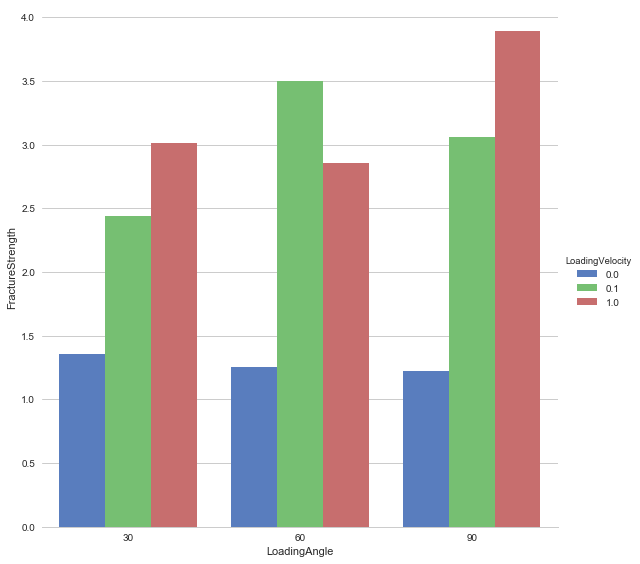
\includegraphics[width=\textwidth]{a.png}
\caption{不同加载速度下的不同角度的断裂强度试验结果:负极} 
\label{fig:a}
\end{figure}
\begin{figure}
\centering   
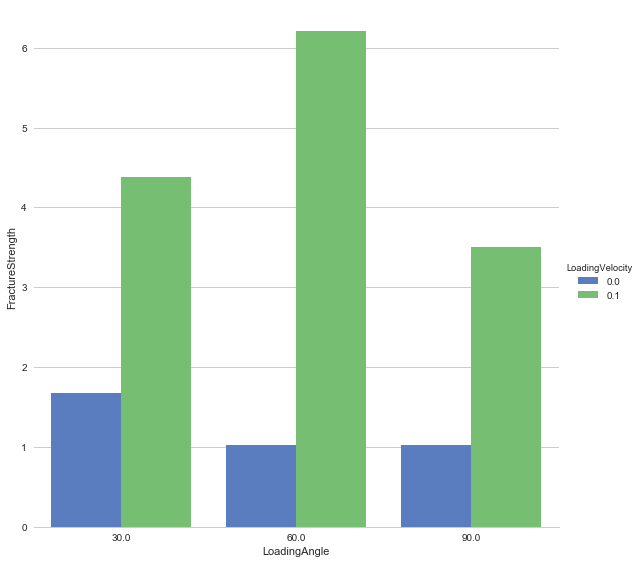
\includegraphics[width=\textwidth]{c.png}
\caption{不同加载速度下的不同角度的断裂强度试验结果:正极} 
\label{fig:c}
\end{figure}

\section{模型建立:力学-化学耦合模型}
在本文的研究中,对于集流体和活性层的宏观测试,无论从实验的断裂面还是从实验测得的实际的断裂强度而言,都表明在电极材料的脱层失效中,颗粒-粘结剂-集流体界面才是最容易发生断裂失效的位置;另一方面,扩散过程中会引起整个活性颗粒乃至胶接表面的应力的重新分布,这是需要在理论和实验研究中需要考虑的关键因素。基于这两点,可以引出对于电池中活性颗粒粘结剂界面力学特性研究的颗粒-壳体模型,其可以综合考量力学和化学因素对于界面力学特性的影响,本文对这一模型在总结中进行介绍和分析,以期能在这一基础上结合本文的研究,进而考虑更加充分的因素改进和修正模型,进行进一步的电池建模研究。
\begin{figure}
\centering   
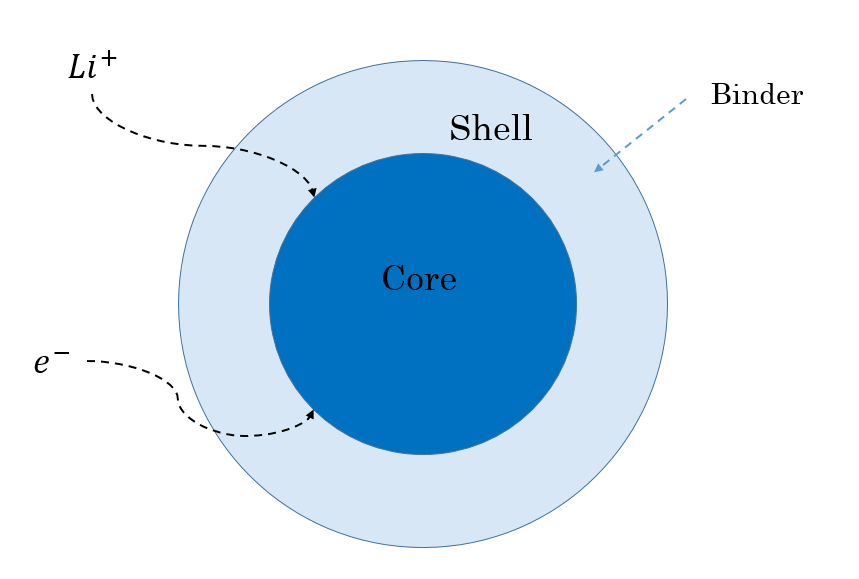
\includegraphics[width=\textwidth]{coreshell.png}
\caption{颗粒-壳体模型示意图。颗粒被粘结剂均匀的包裹,形成外层的壳体,而电子和锂离子在壳体和粘结剂的界面处发生反应,锂离子会进一步向着颗粒内部扩散} 
\label{fig:cs}
\end{figure}
\\
\indent 如图\ref{fig:cs}所示,这一颗粒-壳体模型实际上是由包裹着粘结剂的球形活性颗粒两部分构成。在介绍模型的控制方程之前,需要给定模型的基本假设\cite{Takahashi2016Mechanical}:
\begin{enumerate}
	\item 模型假设活性颗粒之间的相互作用可以忽略并且颗粒之间的电流分布是均匀的。 前一个假设可以由电极活性层的孔隙率保证,而后一个要求电极颗粒的尺寸分布比较均匀和电极的涂布厚度在电极颗粒的尺度误差不大,这些条件在现有的电极生产工艺中可以得到保证\cite{Takahashi2015Examination}。
	\item 不考虑SEI(solid electrolyte interface)膜,即固体电解质界面膜的影响。这一点也被之前对于有着SEI膜影响的活性层的力学性质的实验测定\cite{Zhang2012Direct}和数值模拟\cite{Zheng20143D}所佐证,其影响相对于粘结剂而言可以忽略。
	\item 为了定义边界条件的方便,假定活性颗粒的半径和胶层的厚度在锂离子的脱嵌和嵌入过程中保持不变。 实质上而言,这是一个很强的假设,但是这一假设依然可以给出相当准确的力学分析,因为体积的变化的绝对值还是很小。 但是需要指出的是,进一步的对于硅电极和锡电极的研究中,必须要考虑由于锂离子输运造成的体积变化对于边界条件的影响。
\end{enumerate}
接下来介绍模型的核心理论部分。首先,依据之间的研究\cite{Zhang2007Numerical},给出锂离子在柱坐标中的扩散方程:
\begin{equation}
\label{eq:ch}
\frac{\partial c}{\partial t} = D_s \left( \nabla^2 c -\frac{\Omega}{RT}\nabla c \nabla \sigma_h -\frac{\Omega_c}{RT}\nabla^2 \sigma_h \right)
\end{equation}
其中,$c$是离子密度,$D_s$是扩散系数,$R$是气体常数,$T$是开尔文温度,$\Omega$是锂离子的偏摩尔体积(一定量溶质溶在一摩尔溶液中所引起的体积变化),$\sigma_h$为静水压力。\\
对于力学量,由方程\ref{eq:list1},\ref{eq:list2}和\ref{eq:list3}描述:\\
\begin{align}
\label{eq:list1}
\frac{d \sigma_r}{d r} &+\frac{2}{2}(\sigma_r - \sigma_t)  = 0\\
\label{eq:list2}
\sigma_r =& \frac{E}{(1+\nu)(1-2\nu)} \left[(1-\nu)\frac{d \mu}{d r} +2\nu \frac{\mu}{r} - (1+\nu)\frac{\Delta c \times \Omega}{3} \right] \\
\label{eq:list3}
\sigma_t =& \frac{E}{(1+\nu)(1-2\nu)} \left[\nu\frac{d \mu}{d r} + \frac{\mu}{r} - (1+\nu)\frac{\Delta c \times \Omega}{3} \right]
\end{align}
其中,$\sigma_r$是径向应力分量,$\sigma_t$是切向应力分量,$E$是杨氏模量,$\nu$是泊松比,$\mu$是位移向量,$\Delta c = c-c_0$。\\
方程\ref{eq:ch}为偏微分方程,求解需要给出初始和边界条件:
\begin{align}
c_0=0 \quad & at \quad t=0\\
-D_s\left(\nabla c - \frac{\Omega c}{RT} \nabla \sigma_h \right) = 0 \quad & at \quad r=0\\
-D_s\left(\nabla c - \frac{\Omega c}{RT} \nabla \sigma_h \right) = \frac{i_n}{F} \quad & at \quad r=r_0
\end{align}
同时还有一个自然边界条件:
\begin{equation}
\mu = 0 \quad at \quad r=0
\end{equation}
将颗粒内和胶层内的应力分布联系起来的条件是径向应力在界面处($r=r_0$)的连续性。\\
\indent 接下来,和颗粒内部类似,给出胶层内部的应力分布的控制方程:
\begin{align}
\label{eq:glue1}
\frac{d \sigma_r}{d r} &+ \frac{2}{r}(\sigma_r - \sigma_t) = 0\\
\label{eq:glue2}
\sigma_r =& \frac{E}{(1+\nu)(1-2\nu)}\left[(1-\nu)\frac{d \mu}{d r} + 2\nu \frac{\mu}{r} \right]\\
\label{eq:glue3}
\sigma_t =& \frac{E}{1+\nu}{1-2\nu}\left( \nu\frac{d \mu}{d r}+\frac{u}{r} \right)
\end{align}
值得注意的是,方程\ref{eq:list2}和方程\ref{eq:list3}中的描述锂离子嵌入和脱嵌的第三项没有在方程\ref{eq:glue2}和方程\ref{eq:glue3}中出现。\\
最后给出胶层表面的边界条件:
\begin{equation}
\sigma_r = 0 \quad at \quad r = r_0 + L 
\end{equation}
其中,L是胶层的厚度,这一边界条件实际上说明了没有外力作用。\\
\indent 
依据以上的模型,以求对于界面力学失效行为的微观本质进行模型构建和分析,有着十分重要的意义,接下来我们还将对于前文所没有关注的电化学行为对于电极活性层在颗粒层面的力学特性的影响进行分子模拟的研究,从而从另外一个角度对于这一模型进行完善和补充。
\section{总结和结论}
本章应用设计的混合拉伸-剪切实验方法对于电池正极和负极的活性层-集流体界面胶接强度进行了多种力学加载状况下的测试,并实施了不同速度加载下的动态实验。本章所得到的主要结果如下:
\begin{itemize}
	\item 在拉伸-剪切混合加载实验中,集流体-活性层界面的断裂失效模式会随着剪切分量的变化而发生变化。 其中,在拉伸测试中,主要发生粘接失效,即可以观测到几乎所有的活性层颗粒都会从集流体上脱落。 而在剪切测试中,活性层大多发生相对靠内部的断裂失效,即会有相当一部分活性颗粒继续粘接在集流体上,只有一部分集流体清晰可见。
	\item 在静态多角度加载实验中
	\begin{itemize}
		\item 对正极而言,断裂强度呈现从$1.0MPa$到$2.4MPa$的分布,随着剪切分量的减小(即加载角度从$90^{\circ}$逐渐减小),断裂强度逐渐下降,但是在中间角度如$45^{\circ}$处出现反常取得最值。 总体而言,在较大的剪切分量加载下粘接强度会有所提升。
		\item 对负极而言, 断裂强度要相对小于正极的断裂强度,其分布在$0.9MPa$到$2MPa$之间,并且在$1.25MPa$上下有着明显的集中,推测是由于负极活性层的涂布厚度相对较薄,从而失效模态对应的断裂强度也会比较集中。
	\end{itemize}
	\item 进行的$0.1m/s$和$1m/s$的加载实验表明,动态加载下界面的断裂强度有着显著的提升。 以$0.1m/s$加载为例,对于正极和负极,其不同加载角度下的断裂强度均有着高于两倍的提升。 同时,基于在不同速度加载的比较可以看出其断裂强度随着应变率的变化有着较低的阈值,在加载速度高于一定值($0.1m/s$)后,应变率变化引起的断裂强度的改变不是很明显。 此外,在不同加载速度下,断裂强度随着加载角度的变化也呈现了不同的变化规律。在$0.1m/s$加载速度下,断裂强度呈现先增加后减小的趋势,而在$1m/s$的加载下断裂强度变化呈现相反的趋势。
\end{itemize}

